%%%%%%%%%%%%%%%%%%%%%%%%%%%%%%%%%%%%%%%%%%%%%%%%%%%%%%%%%%%%%%%%%%%%%%%
%% February 10, 2018
%%
%%%%%%%%%%%%%%%%%%%%%%%%%%%%%%%%%%%%%%%%%%%%%%%%%%%%%%%%%%%%%%%%%%%%%%%
\documentclass{article}[12pt,preprint]
\textwidth 17cm
%\textheight 26cm
\hoffset -2.5cm
%\voffset -4.5cm

\usepackage{xcolor,color}
\usepackage{graphicx}
\usepackage{amsmath,amssymb}
\usepackage[colorlinks=true,linkcolor=blue]{hyperref}

\begin{document}

\title{\mbox{\large
	\underline{Proposal for Project at Center for Nuclear Femtography}}
\vspace{0.6cm}
\\ \emph{Navigating the scientific literature with AI}
\vspace{0.2cm}
}

\author{
  N.~Sato$^{1,2}$,
  A. Trewartha$^{3}$ 
	W.~Melnitchouk$^2$,
	I.~C.~Clo\"et$^4$,
	\vspace{0.3cm}
\\
$^1${\it Old Dominion University},
$^2${\it Jefferson Lab},
$^3${\it Berkeley Lab },
\\$^4${\it Argonne National Lab}}

\vspace{-6ex}

%\date{\today}
\date{}

\maketitle

\noindent \color{black}

%%%%%%%%%%%%%%%%%%%%%%%%%%%%%%%%%%%%%%%%%%%%%%%%%%%%%%%%%%%%%%%%%%%%%%%%%
\section{Executive Summary}

Today scientific research in particle and nuclear physics has online
search engines such as inspires, arxive, hepdata to query 
literature and databases.  Such tools are essential in order to
understand and reflect the research in the past in order to look for 
new research directions in the field.  However the amount of
published papers and databases is so big, that in reality the
potential for average scientist in particular newcomers to have a well
informed picture of the field or research topic is very low.  In this
project, we propose to design new tools based on \emph{artificial
intelligence} to boost research productivity similar to those
encountered in the industry such as IBM Watson \cite{...}. 


%%%%%%%%%%%%%%%%%%%%%%%%%%%%%%%%%%%%%%%%%%%%%%%%%%%%%%%%%%%%%%%%%%%%%%%%%
\section{Project outline}
%------------------------------------------------------------------------
\begin{figure}[!h]
\centering
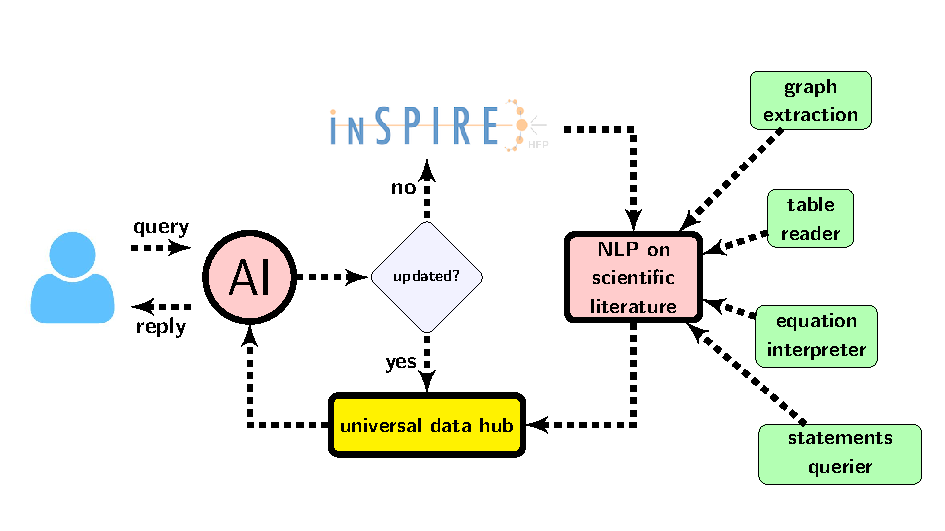
\includegraphics[width=1\textwidth, angle=0]{gallery/ai}  
\caption{Schematic view of the proposal.}
\label{f.1}
\end{figure}

The goal of the project is to build a comprehensive scientific
{\it literature explorer} using artificial intelligence (AI),
tailored for nuclear and high energy particle physics.
%
Currently, a large fraction of researchers' time is invested in 
searching the scientific literature.  The proposed AI will allow
for efficient and automatic extraction of scientific results,
dramatically boosting research productivity.
%
It will be equipped with intelligent decision making tools and 
strategies that will aid the user in exploring and creating insights 
from thousands of scientific papers, highlighting relevant manuscripts 
individualized for each query.
%
For this we plan to:

\begin{itemize}

\item
{\it Design natural language processing} (NLP) {\it algorithms} that
can efficiently interpret the user's queries, as well as automatically
extract relevant information contained in papers in the form of graphs,
tables, equations or scientific statements.  Each of these are
independent skills that can be developed separately.

\item
{\it Construct a database of scientific results} for the AI explorer
to store the collected and processed information from the literature.
The result will be a \emph{universal data hub} (UDH) that can be
regularly updated with the latest scientific results.

\item 
Since the information contained in the literature will be transformed
from the into the UDH internal representation, it avoids the need to
achieve community consensus on standard data storage formats, as well as
allowing efficient integration of historic results.
We will consequently {\it develop apps that can transform and transfer
the information} to the user's desired formats.

\end{itemize}

The project requires an interdisciplinary collaboration with a
machine learning (ML) group from an academic institution that
has expertise in natural language processing algorithms, data
visualization, and data management.  

The completion of the project is a long-term goal, with many subgoals. However we plan to focus in the short-term on creating a queryable database of papers, and the graph extraction capability. This will require the development of software infrastructure to source papers from journal websites, extract plots, and store them in a standardised format on a locally maintained database. This will also involve the development of a UI for the database, allowing its use by the broader research community. 

In the short-term, this will allow users to query plots based on keywords, and in the future, we will extend this application to use ML to interpret graph contents such as axis labels and extract data.

{\color{red}
While the completion of the project is certainly a long-term goal, 
we plan in the short term to focus only on graph extraction capabilities.
This include development of web scraper/paper database that can 
query the arXive based on user defined keywords. In future, we plan to
extend the application to have the AI to interpret  graphs contents 
such as axis labels, legends and units.
}


%%%%%%%%%%%%%%%%%%%%%%%%%%%%%%%%%%%%%%%%%%%%%%%%%%%%%%%%%%%%%%%%%%%%%%%%%
\newpage
\section{Deliverables and timeline}

\begin{itemize}

\item Deliverables:

  \begin{itemize}
  \item Develop data retrieval software for efficiently scraping papers from websites
  \item Develop a local database with appropriate schema for storing data
  \item Develop a UI to facilitate community usage
  \item Develop a software framework for further analysis
  \end{itemize}

\item timeline:

  \begin{itemize}
  \item Mar-Apr: Develop data retrieval software and schema for database
  \item May: Populate local database from web sources
  \item Jun-Jul: Develop a UI for database 
  \item Aug: Web app development
  \item Sep: Web app development
  \end{itemize}

\end{itemize}


%%%%%%%%%%%%%%%%%%%%%%%%%%%%%%%%%%%%%%%%%%%%%%%%%%%%%%%%%%%%%%%%%%%%%%%%%
\newpage
\section{Budget}

\begin{itemize}

\item Personnel:

  \begin{itemize}
  \item M. Kuchera: student support
  \item Y. Li: student support
  \end{itemize}

\item Travel:

  \begin{itemize}
  \item A. Trewartha:  Visit JLab
  \item I. Cloet: Visit JLab
  \item N. Sato:  Visit Argonne 
  \item W. Melnitchouk: Visit Argonne 
  \item N. Sato:  Visit LBNL 
  \item W. Melnitchouk: Visit LBNL
  \end{itemize}

\end{itemize}





%%%%%%%%%%%%%%%%%%%%%%%%%%%%%%%%%%%%%%%%%%%%%%%%%%%%%%%%%%%%%%%%%%%%%%%%%
\begin{thebibliography}{99}

\bibitem{JAM}
Jefferson Lab Angular Momentum (JAM) Collaboration,
{\tt https://www.jlab.org/jam}.

\bibitem{PARTONS}
B.~Berthou {\it et al.},
Eur. Phys. J. C {\bf 78}, 478 (2018).

\end{thebibliography}

\end{document}
